\textbf{04/11/2026 (Clase 14)}
\section{El teorema de Seifert--van Kampen}
\indicetema{t6}

\subsection{Introducción}

Recordemos tres hechos de los temas anteriores.
\begin{enumerate}
    \item[a)] $\pi_1(X)$ es un \textbf{invariante homotópico} de $X$: si $X$ e $Y$ son arco-conexos y $X \simeq Y$, entonces $\pi_1(X) \cong \pi_1(Y)$ (\cref{prop:equiv_homotopica}). Cuando hablamos de $\pi_1(X)$ con $X$ arco-conexo se entiende que elegimos un $x_0 \in X$ cualquiera y que $\pi_1(X) = \pi_1(X,x_0) = C_{x_0}(X)/\!\simeq_{\{0,1\}}$; por el cambio de base (\cref{thm:teo_cambio_base}) no importa qué punto se elija.
    \item[b)] $X$ es simplemente conexo si y solo si $X \neq \emptyset$, $X$ es arco-conexo y $\pi_1(X) = 1$ (\cref{def:def_simp_conexo}).
    \item[c)] El caso particular de dos abiertos de la condición suficiente para que un espacio sea simplemente conexo (\cref{thm:cond_simp_conexo}):
\end{enumerate}

\begin{proposicion}{Condición suficiente con dos abiertos [C14.1]}{svk_dos_abiertos}
Sea $X$ un espacio topológico y sea $\{U, V\}$ un recubrimiento abierto de $X$ tal que:
\begin{enumerate}
    \item[1)] $U$ y $V$ son simplemente conexos;
    \item[2)] $U \cap V$ es arco-conexo;
    \item[3)] $U \cap V \neq \emptyset$.
\end{enumerate}
Entonces $X$ es simplemente conexo.
\end{proposicion}

\begin{proof}
Es el \cref{thm:cond_simp_conexo} con el recubrimiento $\{V_1, V_2\} = \{U, V\}$.
\end{proof}

Este resultado forma parte de una pregunta fundamental: \emph{si lo sabemos todo de unas partes de $X$, ¿qué se puede saber de $X$?} El teorema de Seifert--van Kampen va en esta dirección: calcula $\pi_1(X)$ a partir de los grupos fundamentales de $U$, $V$ y $U \cap V$.

% REVISAR: en el manuscrito pone "Recordemos (6a)"; no está claro a qué ejercicio se refiere.
\begin{observacion}{Recordatorio: lazos homotópicos en $S^1$ [C14.2]}{svk_recordatorio_grado}
Sean $\alpha_1, \alpha_2 \colon I \to S^1$,
\[ \alpha_1(t) = e^{2\pi i (t^2 + t)}, \qquad \alpha_2(t) = e^{2\pi i (a t^2 + b t + c)}, \]
con $a + b,\ c \in \mathbb{Z}$, para que $\alpha_2$ sea un lazo en $1$, como $\alpha_1$. Entonces
\[ \alpha_1 \simeq_{\{0,1\}} \alpha_2 \iff \deg(\alpha_1) = \deg(\alpha_2) \iff a + b = 2. \]
En efecto, $\tilde\alpha_1(t) = t^2 + t$ es una elevación de $\alpha_1$, luego $\deg(\alpha_1) = \tilde\alpha_1(1) - \tilde\alpha_1(0) = 2$; y $\tilde\alpha_2(t) = a t^2 + b t + c$ es una elevación de $\alpha_2$, luego $\deg(\alpha_2) = \tilde\alpha_2(1) - \tilde\alpha_2(0) = a + b$ (\cref{def:def_grado_x0}). La primera equivalencia es el \cref{thm:teo_pi1_s1}.

Si $a + b = 2$, como $c \in \mathbb{Z}$, también $t \mapsto at^2 + bt$ es una elevación de $\alpha_2$, con los mismos extremos ($0$ y $2$) que $\tilde\alpha_1$. Entonces
\[ F \colon I \times I \to S^1, \qquad F(t,\theta) = p\big((1-\theta)(t^2+t) + \theta(at^2+bt)\big), \]
con $p(s) = e^{2\pi i s}$, es una homotopía relativa a $\{0,1\}$ entre $\alpha_1$ y $\alpha_2$. La combinación lineal se hace en $\mathbb{R}$, entre las elevaciones: $(1-\theta)\alpha_1(t) + \theta\alpha_2(t)$ no toma valores en $S^1$ en general.
\end{observacion}
% REVISAR: en el manuscrito aparece F(t,θ) = (1-θ)α_1(t) + θα_2(t), que no cae en S^1; la homotopía con las elevaciones está completada.

\subsection{Preliminares de teoría de grupos}

En todo este apartado $G$ es un grupo. Escribimos $1$ tanto para el elemento neutro de $G$ como para el grupo trivial (en notación aditiva, $0$).

\begin{definicion}{Subgrupo [C14.3]}{svk_subgrupo}
Sea $\emptyset \neq H \subseteq G$. Diremos que $H$ es un \textbf{subgrupo} de $G$, y escribiremos $H \leq G$, cuando
\[ 1 \in H, \qquad gh \in H \ \ \forall g, h \in H, \qquad g^{-1} \in H \ \ \forall g \in H. \]
Equivalentemente, $gh^{-1} \in H$ para todo $g, h \in H$.
\end{definicion}

\begin{proof}[Demostración de la equivalencia]
$\Rightarrow)$ Claro. $\Leftarrow)$ Como $H \neq \emptyset$, sea $g \in H$: $gg^{-1} \in H$, es decir, $1 \in H$. Entonces $1 \cdot g^{-1} = g^{-1} \in H$ para todo $g \in H$. Por último, si $g, h \in H$, entonces $h^{-1} \in H$ y $g (h^{-1})^{-1} = gh \in H$.
\end{proof}

\begin{definicion}{Subgrupo generado [C14.4]}{svk_generado}
Sea $S \subseteq G$. El \textbf{subgrupo generado} por $S$ es
\[ \langle S \rangle := \bigcap_{\substack{H \leq G \\ S \subseteq H}} H, \]
el menor subgrupo de $G$ que contiene a $S$. Es sencillo probar que
\[ \langle S \rangle = \{ g_1^{n_1} g_2^{n_2} \cdots g_r^{n_r} : g_1, \dots, g_r \in S,\ n_1, \dots, n_r \in \mathbb{Z},\ r \geq 0 \}. \]
\end{definicion}

\begin{definicion}{Subgrupo normal [C14.5]}{svk_normal}
Sea $H \leq G$. Diremos que $H$ es \textbf{normal} en $G$, y escribiremos $H \trianglelefteq G$, cuando $ghg^{-1} \in H$ para todo $h \in H$ y todo $g \in G$. El elemento $ghg^{-1}$ es el \textbf{conjugado} de $h$ por $g$.
\end{definicion}

Sea $H \leq G$ y consideremos en $G$ la relación
\[ g_1 \sim g_2 \iff g_1 g_2^{-1} \in H. \]
Es una relación binaria de equivalencia, así que podemos hablar del conjunto cociente $G/\!\sim$. Intentamos dotarlo de estructura de grupo con la operación
\[ G/\!\sim \times\, G/\!\sim \;\longrightarrow\; G/\!\sim, \qquad ([g],[h]) \longmapsto [gh]. \]

\begin{teorema}{Grupo cociente [C14.6] \marcaE}{svk_cociente}
La operación anterior está bien definida (es decir, $g \sim g'$ y $h \sim h'$ implican $gh \sim g'h'$) si y solo si $H \trianglelefteq G$.

En consecuencia, si $H \trianglelefteq G$ podemos hablar del \textbf{grupo cociente} $G/\!\sim$, que denotaremos por $G/H$.
\end{teorema}

\begin{proof}
(Se propuso como ejercicio; la demostración está completada.)

$\Leftarrow)$ Si $g g'^{-1} \in H$ y $h h'^{-1} \in H$, entonces
\[ gh\,(g'h')^{-1} = g\,(h h'^{-1})\,g^{-1} \cdot g g'^{-1} \in H, \]
porque $g (hh'^{-1}) g^{-1} \in H$ por ser $H$ normal, y $H$ es cerrado para el producto.

$\Rightarrow)$ Sean $h \in H$ y $g \in G$. Como $h \cdot 1^{-1} = h \in H$, se tiene $h \sim 1$; y $g \sim g$. Por la buena definición, $gh \sim g \cdot 1 = g$, es decir, $gh g^{-1} \in H$.
\end{proof}

\begin{definicion}{Conmutador de un grupo [C14.7]}{svk_conmutador}
El \textbf{conmutador} de $G$ es el subgrupo generado por los conmutadores de sus elementos:
\[ [G,G] := \big\langle \{ g_1 g_2 g_1^{-1} g_2^{-1} : g_1, g_2 \in G \} \big\rangle. \]
\end{definicion}

\begin{observacion}{[C14.8]}{svk_abeliano_conmutador}
$G$ es abeliano si y solo si $[G,G] = 1$, porque $g_1 g_2 g_1^{-1} g_2^{-1} = 1 \iff g_1 g_2 = g_2 g_1$.
\end{observacion}

\begin{teorema}{Abelianizado [C14.9] \marcaE}{svk_abelianizado}
Sea $G$ un grupo. Entonces:
\begin{enumerate}
    \item[a)] $[G,G] \trianglelefteq G$, así que podemos hablar del grupo $G/[G,G]$.
    \item[b)] $G/[G,G]$ siempre es abeliano.
    \item[c)] Si $N \trianglelefteq G$ y $G/N$ es abeliano, entonces $[G,G] \subseteq N$.
\end{enumerate}
Equivalentemente, $[G,G]$ es el menor subgrupo normal de $G$ cuyo cociente es abeliano (véase Rotman).
\end{teorema}

\begin{proof}
(En clase se enunciaron a) y b) sin demostración y c) se propuso como ejercicio; la demostración de c) está completada.)

c) Sean $g_1, g_2 \in G$. Como $G/N$ es abeliano, $[g_1][g_2] = [g_2][g_1]$, es decir, $[g_1 g_2 g_1^{-1} g_2^{-1}] = [1]$, luego $g_1 g_2 g_1^{-1} g_2^{-1} \in N$. Así $N$ es un subgrupo que contiene a todos los conmutadores, y por tanto contiene al subgrupo que generan: $[G,G] \subseteq N$.
\end{proof}

\begin{definicion}{Subgrupo normal generado [C14.10]}{svk_normal_generado}
Sea $S \subseteq G$. El \textbf{subgrupo normal de $G$ generado por $S$} es
\[ \langle\langle S \rangle\rangle := \bigcap_{\substack{H \trianglelefteq G \\ S \subseteq H}} H \;\supseteq\; \langle S \rangle = \bigcap_{\substack{H \leq G \\ S \subseteq H}} H, \]
el menor subgrupo normal de $G$ que contiene a $S$.
\end{definicion}

\begin{teorema}{Descripción de $\langle\langle S \rangle\rangle$ [C14.11]}{svk_normal_generado_desc}
Sea $S \subseteq G$ y, para $h \in G$, sea $c_h \colon G \to G$ la conjugación $c_h(g) = h g h^{-1}$. Entonces
\[ \langle\langle S \rangle\rangle = \big\{ c_{h_1}(g_1^{n_1})\, c_{h_2}(g_2^{n_2}) \cdots c_{h_r}(g_r^{n_r}) \big\}, \]
con $g_1, \dots, g_r \in S$, $n_1, \dots, n_r \in \mathbb{Z}$, $h_1, \dots, h_r \in G$ y $r \geq 0$.
Compárese con $\langle S \rangle = \{ g_1^{n_1} \cdots g_r^{n_r} : g_i \in S,\ n_i \in \mathbb{Z},\ r \geq 0 \}$ (\cref{def:svk_generado}).
\end{teorema}

\subsection{Grupos libres}

\begin{definicion}{Palabras [C14.12]}{svk_palabras}
Sea $S$ un conjunto cualquiera.
\begin{enumerate}
    \item[a)] Una \textbf{palabra} en $S$ es una yuxtaposición $g_1^{\varepsilon_1} g_2^{\varepsilon_2} \cdots g_r^{\varepsilon_r}$ con $g_1, \dots, g_r \in S$ y $\varepsilon_1, \dots, \varepsilon_r \in \{-1, 1\}$.
    \item[b)] La \textbf{palabra vacía} es aquella en la que no aparece ningún elemento de $S$. La denotaremos por $1$.
    \item[c)] Una palabra es \textbf{reducida} cuando no tiene dos símbolos consecutivos de la forma $a a^{-1}$ ni $a^{-1} a$, con $a \in S$.
    \item[d)] Una \textbf{palabra generalizada} es $g_1^{n_1} g_2^{n_2} \cdots g_r^{n_r}$ con $n_1, \dots, n_r \in \mathbb{Z} \setminus \{0\}$. En la forma reducida de las palabras generalizadas no hay términos consecutivos de la forma $a^{\varepsilon_1} a^{\varepsilon_2}$: se agrupan en una potencia.
\end{enumerate}
Por ejemplo,
\[ abcbbc^{-1}ba^{-1}abbc = abcb^2c^{-1}bbb\,c = \underbrace{abcb^2c^{-1}b^3c}_{\text{reducida}}. \]
\end{definicion}
% REVISAR: en el manuscrito c) tiene dos condiciones numeradas 1) y 2); la segunda (agrupar a^e1 a^e2) se ha pasado a d), que es donde se usan los exponentes.

\begin{definicion}{Grupo libre [C14.13]}{svk_grupo_libre}
Sea $S \neq \emptyset$. $F(S)$ es el conjunto de las palabras reducidas formadas con los elementos de $S$, con la operación de yuxtaponer y reducir. Es el \textbf{grupo libre generado por $S$}. Si $S$ es finito, se dice que $F(S)$ tiene \textbf{rango} $|S| = \#S$; escribimos $F_n$ para el grupo libre de rango $n$. A los grupos $F(S)$ se les llama \textbf{grupos libres}.
\end{definicion}

\begin{observacion}{Ejemplos de grupos libres [C14.14]}{svk_ej_libres}
\begin{itemize}
    \item Si $S = \{a, b\}$, entonces $F(S) = \{1, a, a^2, a^{-1}, \dots, b, b^2, b^{-1}, \dots, ab, ab^2, a^2b, a^{-1}b, \dots\}$. Veremos que el grupo fundamental de la figura ocho $S^1 \vee S^1$ (\cref{def:def_wedge}), con un lazo $a$ y un lazo $b$ que recorren cada circunferencia, es $\pi_1(S^1 \vee S^1) = F(\{a,b\})$ (\cref{obs:svk_ej_ocho_toro}).
    \item $F_1 = F(\{a\}) = \{1, a, a^{-1}, a^{n_1} a^{n_2} \cdots a^{n_r} = a^{n_1 + \dots + n_r}\} = \{a^n : n \in \mathbb{Z}\} \cong \mathbb{Z}$, mediante el isomorfismo $\mathbb{Z} \to F(\{a\})$, $n \mapsto a^n$.
\end{itemize}
\end{observacion}

\begin{definicion}{Grupo abeliano libre [C14.15]}{svk_abeliano_libre}
Sea $S \neq \emptyset$. El \textbf{grupo abeliano libre} $F_0(S)$ (también $F^{ab}(S)$) es el grupo cuyo soporte son las palabras reducidas formadas con los elementos de $S$, permitiendo la conmutatividad. Por ejemplo,
\[ F_0(\{a, b\}) = \{a^n b^m : n, m \in \mathbb{Z}\} \cong \mathbb{Z} \times \mathbb{Z}, \]
mediante $\mathbb{Z} \times \mathbb{Z} \to F_0(\{a,b\})$, $(n,m) \mapsto a^n b^m$.
En general, si $\#S = n$, entonces $F_0(S) \cong \mathbb{Z}^n$.
\end{definicion}

\begin{observacion}{Diferencia entre $F$ y $F_0$ [C14.16]}{svk_F_F0}
$F(\{a,b\}) \not\cong F_0(\{a,b\})$: el segundo es abeliano y el primero no ($ab$ y $ba$ son palabras reducidas distintas). Topológicamente,
\[ \pi_1(S^1 \vee S^1) \cong F(\{a,b\}) \not\cong F_0(\{a,b\}) \cong \mathbb{Z} \times \mathbb{Z} \cong \pi_1(T^2), \]
donde la última igualdad es la \cref{prop:ej_pi1_producto}. En particular, la figura ocho y el toro no tienen el mismo tipo de homotopía.
\end{observacion}

\begin{proposicion}{Lema: abelianizado de un grupo libre [C14.17]}{svk_lema_F0}
Sea $S \neq \emptyset$. Entonces $F_0(S) \cong F(S)/[F(S), F(S)]$.
\end{proposicion}

\begin{teorema}{Rango de un grupo libre [C14.18]}{svk_rango}
Sean $n, m \in \mathbb{Z}_{\geq 1}$. Entonces $F_n \cong F_m \iff n = m$.
\end{teorema}

\begin{proof}
$\Leftarrow)$ Claro. $\Rightarrow)$ Un isomorfismo $F_n \cong F_m$ lleva conmutadores en conmutadores, luego lleva $[F_n,F_n]$ en $[F_m,F_m]$ e induce un isomorfismo entre los abelianizados. Por el \cref{prop:svk_lema_F0},
\[ \mathbb{Z}^n \cong F_0(S_n) \cong \frac{F_n}{[F_n,F_n]} \cong \frac{F_m}{[F_m,F_m]} \cong F_0(S_m) \cong \mathbb{Z}^m. \]
Un isomorfismo $\mathbb{Z}^n \cong \mathbb{Z}^m$ lleva $2\mathbb{Z}^n$ en $2\mathbb{Z}^m$, así que
\[ \Big(\frac{\mathbb{Z}}{2\mathbb{Z}}\Big)^n \cong \frac{\mathbb{Z}^n}{2\mathbb{Z}^n} \cong \frac{\mathbb{Z}^m}{2\mathbb{Z}^m} \cong \Big(\frac{\mathbb{Z}}{2\mathbb{Z}}\Big)^m. \]
Ambos son espacios vectoriales sobre el cuerpo $\mathbb{Z}/2\mathbb{Z}$, de dimensiones $n$ y $m$, y son isomorfos, luego $n = m$.
\end{proof}

\begin{teorema}{Todo grupo es imagen epimorfa de un grupo libre [C14.19]}{svk_epimorfismo}
Sea $G$ un grupo. Entonces existen un grupo libre $F$ y un epimorfismo $\varphi \colon F \to G$. Además, $F$ puede tomarse como $F(S)$ para cualquier sistema generador $S$ de $G$.
\end{teorema}

\begin{proof}
Sea $S$ cualquier sistema generador de $G$, es decir, $\langle S \rangle = G$, y por la \cref{def:svk_generado}
\[ G = \langle S \rangle = \{ g_1^{n_1} \cdots g_r^{n_r} : g_1, \dots, g_r \in S,\ n_1, \dots, n_r \in \mathbb{Z},\ r \geq 0 \}. \]
Sea $F = F(S)$ y definimos
\[ \varphi \colon F \to G, \qquad \underbrace{g_1^{n_1} g_2^{n_2} \cdots g_r^{n_r}}_{\text{yuxtaposición}} \longmapsto \underbrace{g_1^{n_1} g_2^{n_2} \cdots g_r^{n_r}}_{\text{producto en } G}. \]
Es un homomorfismo (yuxtaponer y reducir en $F$ corresponde a multiplicar en $G$) y es sobreyectivo porque todo elemento de $G$ es un producto de ese tipo. Luego $\varphi$ es un epimorfismo.
\end{proof}

\begin{observacion}{El núcleo es normal [C14.20]}{svk_nucleo_normal}
Si $\varphi \colon G_1 \to G_2$ es un homomorfismo de grupos, entonces $K = \ker(\varphi) \trianglelefteq G_1$. En efecto, para $h \in K$ y $g \in G_1$,
\[ \varphi(ghg^{-1}) = \varphi(g)\varphi(h)\varphi(g^{-1}) = \varphi(g)\varphi(g^{-1}) = \varphi(1) = 1, \]
luego $ghg^{-1} \in K$. Como consecuencia del \cref{thm:svk_epimorfismo} y del primer teorema de isomorfía,
\[ F/\ker(\varphi) \cong G. \]
\end{observacion}

\bigskip
\textbf{06/11/2026 (Clase 15)}

\subsection{Presentaciones y producto libre}

Como consecuencia de la \cref{obs:svk_nucleo_normal}: si disponemos de un sistema generador $S$ de $G$ y de un conjunto $R$ que genera $\ker(\varphi)$ (como subgrupo normal, $\langle\langle R \rangle\rangle = \ker(\varphi)$), automáticamente $G$ está unívocamente determinado:
\[ G \cong F(S) / \langle\langle R \rangle\rangle. \]

\begin{definicion}{Presentación de un grupo [C15.1]}{svk_presentacion}
Con la notación anterior se escribe $G = \langle S ; R \rangle$, y se dice que $G$ está \textbf{presentado por generadores y relaciones}. Recordemos que $\varphi \colon F(S) \to G$ manda la yuxtaposición $g_1^{r_1} \cdots g_m^{r_m}$ ($g_i \in S$, $r_i \in \mathbb{Z}$) al producto $g_1^{r_1} \cdots g_m^{r_m}$ en $G$.
\end{definicion}

\begin{observacion}{Ejemplos de presentaciones [C15.2]}{svk_ej_presentaciones}
\begin{enumerate}
    \item[1)] $F_1 = \mathbb{Z} = \langle a ; \ \rangle$ (sin relaciones).
    \item[2)] $\mathbb{Z}^2 = \mathbb{Z} \times \mathbb{Z} = \langle a, b ; aba^{-1}b^{-1} \rangle$.
    \item[3)] $\mathbb{Z}/5\mathbb{Z} = \langle a ; a^5 \rangle$.
\end{enumerate}
\end{observacion}

\begin{definicion}{Producto libre de grupos [C15.3]}{svk_producto_libre}
Sean $G_1 = \langle S_1 ; R_1 \rangle$ y $G_2 = \langle S_2 ; R_2 \rangle$. Su \textbf{producto libre} es
\[ G_1 * G_2 := \langle S_1 \cup S_2 ; R_1 \cup R_2 \rangle. \]
Si $S_1 = \{g_1, g_2, \dots\}$ y $S_2 = \{h_1, h_2, \dots\}$, los elementos de $G_1 * G_2$ son palabras como $g_1^5 g_4^{-1} h_1 g_2 h_2 h_3^7 g_5 h_7$: los símbolos consecutivos de $G_1$ se operan en $G_1$, los de $G_2$ en $G_2$, y entre unos y otros se concatena.
\end{definicion}
% REVISAR: se entiende S_1 y S_2 disjuntos (unión disjunta) aunque en el papel pone S_1 ∪ S_2.

\begin{observacion}{Ejemplos de productos libres [C15.4]}{svk_ej_producto_libre}
\begin{itemize}
    \item $\mathbb{Z} * \mathbb{Z} = \langle a ; \ \rangle * \langle b ; \ \rangle = \langle a, b ; \ \rangle = F(\{a,b\}) = F_2$.
    \item $\mathbb{Z} * \mathbb{Z} * \mathbb{Z} = \langle a, b, c ; \ \rangle = F_3$.
    \item En cambio, $\mathbb{Z} \times \mathbb{Z} = \langle a, b ; aba^{-1}b^{-1} \rangle$, mientras que $\mathbb{Z} * \mathbb{Z} = \langle a, b ; \ \rangle$.
\end{itemize}
\end{observacion}

\subsection{Push-out de grupos y el teorema de Seifert--van Kampen}

\begin{teorema}{Push-out de grupos [C15.5]}{svk_pushout}
Consideremos un diagrama de homomorfismos de grupos $\varphi_1 \colon H \to G_1$, $\varphi_2 \colon H \to G_2$. Entonces existe una \textbf{completación} de este diagrama, un grupo $\mathcal{G}$ con homomorfismos $\psi_1 \colon G_1 \to \mathcal{G}$ y $\psi_2 \colon G_2 \to \mathcal{G}$ tales que $\psi_1 \circ \varphi_1 = \psi_2 \circ \varphi_2$, de forma que: para todo grupo $G$ y todos los homomorfismos $s_1 \colon G_1 \to G$, $s_2 \colon G_2 \to G$ con $s_1 \circ \varphi_1 = s_2 \circ \varphi_2$, existe un único homomorfismo $f \colon \mathcal{G} \to G$ con
\[ s_1 = f \circ \psi_1 \qquad \text{y} \qquad s_2 = f \circ \psi_2. \]
\begin{center}
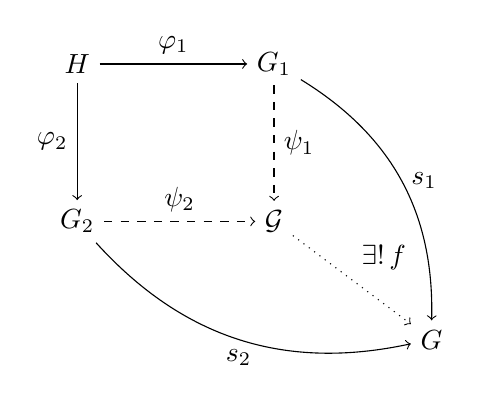
\begin{tikzpicture}
\node (H) at (0,2) {$H$};
\node (G1) at (2.5,2) {$G_1$};
\node (G2) at (0,0) {$G_2$};
\node (P) at (2.5,0) {$\mathcal{G}$};
\node (G) at (4.5,-1.5) {$G$};
\draw[->] (H) -- (G1) node[midway, above] {$\varphi_1$};
\draw[->] (H) -- (G2) node[midway, left] {$\varphi_2$};
\draw[->, dashed] (G1) -- (P) node[midway, right] {$\psi_1$};
\draw[->, dashed] (G2) -- (P) node[midway, above] {$\psi_2$};
\draw[->] (G1) to[bend left=30] node[midway, right] {$s_1$} (G);
\draw[->] (G2) to[bend right=30] node[midway, below] {$s_2$} (G);
\draw[->, dotted] (P) -- (G) node[midway, above right] {$\exists!\, f$};
\end{tikzpicture}
\end{center}
En la prueba de este resultado se ve que $\mathcal{G}$ es único salvo isomorfismo: es el \textbf{push-out} de $\varphi_1$ y $\varphi_2$. Además, si $G_1 = \langle S_1 ; R_1 \rangle$, $G_2 = \langle S_2 ; R_2 \rangle$ y $H = \langle S ; R \rangle$, entonces
\[ \mathcal{G} \cong \frac{G_1 * G_2}{N} \cong \langle S_1 \cup S_2 ; R_1 \cup R_2 \cup R_0 \rangle, \]
con $R_0 = \{ \varphi_1(h)\varphi_2(h)^{-1} : h \in S \}$, donde $N$ es el subgrupo normal de $G_1 * G_2$ generado por $R_0$.
\end{teorema}
% REVISAR: en el manuscrito los nombres psi_1 y psi_2 están cruzados (psi_2: G_1 -> G, psi_1: G_2 -> G); aquí psi_k sale de G_k.

\begin{teorema}{de Seifert--van Kampen [C15.6]}{svk_teorema}
Sea $X$ un espacio topológico, sea $x_0 \in X$ y sea $\{U, V\}$ un recubrimiento abierto de $X$. Supongamos que $X$, $U$, $V$ y $U \cap V$ son arco-conexos y que $x_0 \in U \cap V$. Sean $i_1 \colon U \cap V \to U$, $i_2 \colon U \cap V \to V$, $j_1 \colon U \to X$ y $j_2 \colon V \to X$ las inclusiones, que forman un diagrama conmutativo ($j_1 \circ i_1 = j_2 \circ i_2$). Entonces el diagrama inducido
\begin{center}
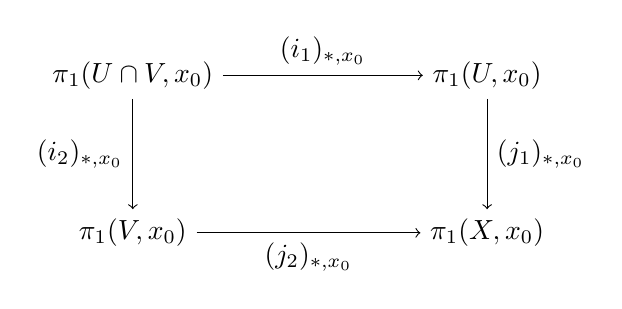
\begin{tikzpicture}
\node (A) at (0,2) {$\pi_1(U \cap V, x_0)$};
\node (B) at (4.5,2) {$\pi_1(U, x_0)$};
\node (C) at (0,0) {$\pi_1(V, x_0)$};
\node (D) at (4.5,0) {$\pi_1(X, x_0)$};
\draw[->] (A) -- (B) node[midway, above] {$(i_1)_{*,x_0}$};
\draw[->] (A) -- (C) node[midway, left] {$(i_2)_{*,x_0}$};
\draw[->] (B) -- (D) node[midway, right] {$(j_1)_{*,x_0}$};
\draw[->] (C) -- (D) node[midway, below] {$(j_2)_{*,x_0}$};
\end{tikzpicture}
\end{center}
también conmuta y es un diagrama push-out. Por el \cref{thm:svk_pushout}, si $\pi_1(U,x_0) = \langle S_1 ; R_1 \rangle$, $\pi_1(V,x_0) = \langle S_2 ; R_2 \rangle$ y $\pi_1(U \cap V, x_0) = \langle S ; R \rangle$, entonces
\[ \pi_1(X, x_0) \cong \langle S_1 \cup S_2 ; R_1 \cup R_2 \cup R_0 \rangle, \]
con $R_0 = \{ (i_1)_*(h)\,\big((i_2)_*(h)\big)^{-1} : h \in S \}$.
\end{teorema}
% REVISAR: en el manuscrito pone "U ∩ X arcoconexos" (se entiende U ∩ V) y "x_0 ∈ U ∪ V" (se entiende U ∩ V, que es donde está el punto base de pi_1(U ∩ V, x_0)).
% La conmutatividad del diagrama inducido sale de la funtorialidad de los homomorfismos inducidos (\cref{thm:teo_hom_ind}).

\begin{observacion}{La figura ocho y la rosa de $n$ pétalos [C15.7]}{svk_ej_ocho_toro}
Sea $X = S^1 \vee S^1$ la figura ocho y $x_0$ el punto de unión. Tomamos $U$ = $X$ menos un punto de la circunferencia de la derecha y $V$ = $X$ menos un punto de la de la izquierda. Entonces $U \simeq S^1$, $V \simeq S^1$ y $U \cap V$ es una cruz, contráctil, así que
\[ \pi_1(U \cap V, x_0) = 1, \quad \pi_1(U, x_0) = \mathbb{Z} = \langle b ; \ \rangle, \quad \pi_1(V, x_0) = \mathbb{Z} = \langle a ; \ \rangle, \]
y por el \cref{thm:svk_teorema}, $\pi_1(X, x_0) = \langle a, b ; \ \rangle \cong F_2$.

La \textbf{$n$-rosa} es el ramo de $n$ circunferencias $\bigvee_n S^1$ (\cref{def:def_wedge}), también llamado \emph{bouquet} de esferas. Aplicando inducción se llega a que $\pi_1\big(\bigvee_n S^1\big) \cong F_n$.
\end{observacion}

\begin{observacion}{Un toro con el agujero central reducido a un punto [C15.8]}{svk_ej_toro_cornudo}
% REVISAR: el espacio X solo está dibujado. Parece el toro que se obtiene girando alrededor del eje z una circunferencia tangente al eje (el agujero central se reduce a un punto, donde está dibujado x_0 en el primer dibujo).
Sea $X$ el toro que se obtiene al girar alrededor del eje $z$ una circunferencia tangente a dicho eje, sea $p \in X$ un punto (distinto del punto del eje) y sea $x_0 \neq p$ con $x_0 \in U \setminus \{p\}$, de modo que $x_0 \in U \cap V$, donde
\[ U = B(p, \varepsilon) \cap X \ \ (\varepsilon > 0 \text{ suficientemente pequeño}), \qquad V = X \setminus \{p\}. \]
Entonces $U$ es un disco ($\pi_1(U,x_0) = 1$), $U \cap V$ es un disco sin un punto ($\pi_1(U \cap V, x_0) \cong \mathbb{Z} = \langle a ; \ \rangle$) y $\pi_1(V, x_0) = \langle b ; \ \rangle \cong \mathbb{Z}$. El lazo $a$ alrededor de $p$ es trivial en $V$: $(i_2)_{*}(a) = bb^{-1} = 1$. Por el \cref{thm:svk_teorema}, con $R_0 = \{ (i_1)_*(a)\,((i_2)_*(a))^{-1} \}$,
\[ \pi_1(X, x_0) \cong \big\langle b ; \underbrace{(i_1)_*(a)}_{1} \underbrace{\big((i_2)_*(a)\big)^{-1}}_{(bb^{-1})^{-1} = 1} \big\rangle = \langle b ; \ \rangle \cong \mathbb{Z}. \]
\end{observacion}
% REVISAR: a continuación hay un ejemplo 3) con un dibujo de una región con un agujero sombreado y "≅ Z"; no se ha podido identificar el espacio.

\begin{observacion}{El grupo fundamental del toro por Seifert--van Kampen [C15.9]}{svk_ej_toro}
Ya sabemos que $\pi_1(T^2) = \mathbb{Z} \times \mathbb{Z}$ (\cref{prop:ej_pi1_producto}). Veamos que también se puede deducir del \cref{thm:svk_teorema}. Sean $X = T^2$, $p \in X$ y
\[ U = B(p, \varepsilon) \cap X \ \ (\varepsilon > 0 \text{ suficientemente pequeño}), \qquad V = X \setminus \{p\}, \]
con $x_0 \in U \cap V$. Entonces:
\begin{itemize}
    \item $U \cap V$ es un disco sin un punto, $U \cap V \simeq S^1$, y $\pi_1(U \cap V, x_0) = \langle a ; \ \rangle$, ya que $\pi_1(S^1) = \langle 1 \rangle$ vía el grado, $\deg \colon \pi_1(S^1) \to \mathbb{Z} = \langle 1 \rangle$ (\cref{thm:teo_pi1_s1}).
    \item $U$ es un disco, así que $\pi_1(U, x_0) = 1$.
    \item $V = T^2 \setminus \{p\}$ se retrae sobre dos circunferencias $b$ y $c$ unidas por un punto, una figura ocho, así que $\pi_1(V, x_0) \cong F_2 = \langle b, c ; \ \rangle$.
\end{itemize}
El lazo $a$, que rodea a $p$, recorre en $V$ el borde del cuadrado con el que se construye el toro, así que $(i_2)_*(a) = cbc^{-1}b^{-1}$, y $(i_1)_*(a) = 1$. Por tanto
\[ \pi_1(T^2, x_0) = \langle b, c ; cbc^{-1}b^{-1} \rangle \cong \mathbb{Z} \times \mathbb{Z}. \]
\end{observacion}
% REVISAR: el valor (i_2)_*(a) = cbc^{-1}b^{-1} (y la explicación del borde del cuadrado) está completado; en el papel solo aparece el resultado <b, c; cbc^{-1}b^{-1}>.

\begin{observacion}{Otras superficies [C15.10]}{svk_ej_superficies}
En clase se dibujaron además: una superficie (esfera con varios agujeros) que se retrae sobre una rosa de $6$ pétalos, cuyo grupo fundamental es por tanto $F_6$, y el bitoro y el tritoro (superficies de género $2$ y $3$).
\end{observacion}
% REVISAR: los dibujos de la última página no llevan cálculos; el número de agujeros de la primera superficie no se distingue bien (el resultado anotado es F_6).
